\documentclass[11pt,twoside]{article}
\usepackage{asp2010}
\usepackage{graphicx}

\resetcounters 

\markboth{Christopher P.\ L.\ Berry and Jonathan R.\ Gair}{EMRBs from the Galactic Centre}

\begin{document}

\resetcounters

\title{Extreme-mass-ratio bursts from the Galactic Centre}
 \author{Christopher~P.~L.~Berry and Jonathan R.\ Gair \affil{Institute of Astronomy, University of Cambridge, Cambridge, UK}}
 
\begin{abstract} 
An extreme-mass-ratio burst (EMRB) is a gravitational wave signal emitted when a compact object passes through periapsis on a highly eccentric orbit about a much more massive object, in our case a stellar mass object about the $4.31 \times 10^6 M_\odot$ massive black hole (MBH) in the Galactic Centre. We investigation how EMRBs could allow us to constrain the parameters of the Galaxy's MBH. EMRBs should be detectable if the periapse distance is $r_\mathrm{p} < 65 r_\mathrm{g}$ for a $\mu = 10 M_\odot$ orbiting object, where $r_\mathrm{g} = GM_\bullet/c^2$ is the gravitational radius. The signal-to-noise ratio scales approximately as $\log(\rho) \simeq -2.7\log(r_\mathrm{p}/r_\mathrm{g}) + \log(\mu/M_\odot) + 4.9$. For periapses smaller than $\sim 10 r_\mathrm{g}$, EMRBs can be informative, providing good constraints on both the MBH's mass and spin.
\end{abstract}

\section{Introduction} 

We currently believe that most galactic nuclei have harboured a massive black hole (MBH) during their evolution~\citep{Lynden-Bell1971, Soltan1982, Rees1984}. Observations have shown there are correlations between the MBHs' masses and their host galaxies' properties, such as bulge luminosity, mass, velocity dispersion and light concentration~\citep{Kormendy1995, Magorrian1998, Ferrarese2000, Gebhardt2000, Graham2001, Tremaine2002, Marconi2003, Haring2004, Graham2007, Graham2011}. These suggest coeval evolution of the MBH and galaxy~\citep{Peng2007, Jahnke2011}, possibly with feedback mechanisms coupling the two~\citep{Haiman2004, Volonteri2009}. The MBH and the surrounding spheroidal galaxy share a common history, such that one can inform us of the other.

The best opportunity to study MBHs comes from the compact object in our own galactic centre (GC), which is coincident with Sagittarius A* (Sgr A*). Through careful monitoring of stars orbiting the GC, this has been identified as an MBH of mass $M_\bullet = 4.31 \times 10^6 M_\odot$ at a distance of only $R_0 = 8.33~\mathrm{kpc}$~\citep{Gillessen2009}.

According to the no-hair theorem, the MBH should be described completely by just its mass $M_\bullet$ and spin $a$\citep{Israel1967, Israel1968, Carter1971, Hawking1972, Robinson1975, Chandrasekhar1998}. The (dimensionless) spin parameter $a_\ast$ is related to the BH's angular momentum $J$ by
\begin{equation}
a_\ast = \frac{cJ}{GM_\bullet^2}.
\end{equation}
As we have a good estimate of the mass, to gain a complete description of the MBH we have only to measure its spin.

The spin of is determined by several competing processes. An MBH accumulates mass and angular momentum through accretion~\citep{Volonteri2010}. Accretion from a gaseous disc shall spin up the MBH, potentially leading to high spin values~\citep{Volonteri2005}. A series of randomly orientated accretion events shall lead to a low spin value: we expect an average value $|a_\ast| \sim 0.1$--$0.3$~\citep*{King2006, King2008}. The MBH shall also grow through mergers~\citep{Yu2002, Malbon2007}. Minor mergers with smaller black holes (BHs) can decrease the spin~\citep*{Hughes2003, Gammie2004}. A series of major mergers, between similar mass MBHs, would lead to a likely spin of $|a_\ast| \sim 0.69$~\citep{Berti2008, Berti2007, Gonzalez2007}. Measuring the spin of MBHs shall help us understand the relative importance of these processes, and gain insight into their galaxies' pasts.

An exciting means of inferring information about the MBH is through gravitational waves (GWs) emitted when compact objects (COs), such as stellar mass BHs, neutron stars (NSs), white dwarfs (WDs) or low mass main sequence (MS) stars, pass close by~\citep{Sathyaprakash2009}. A space-borne detector, such as the \textit{Laser Interferometer Space Antenna} (\textit{LISA}) or the \textit{evolved Laser Interferometer Space Antenna} (\textit{eLISA}), can detect GWs in the frequency range of interest for these encounters~\citep{Bender1998, Danzmann2003, Jennrich2011, Amaro-Seoane2012a}. Much work has already been done on the waveforms generated when companion objects inspiral towards an MBH~\citep{Glampedakis2005, Barack2009}. The initial orbits may be highly elliptical and a burst of radiation is emitted during each close encounter. These are known as extreme mass-ratio bursts (EMRBs; \citealt{Rubbo2006}). Assuming that the companion is not scattered from its orbit, and does not plunge straight into the MBH, its orbit shall evolve, becoming more circular, and it shall begin to continuously emit significant gravitational radiation in the \textit{LISA}/\textit{eLISA} frequency range. The resulting signals are known as extreme mass-ratio inspirals (EMRIs; \citealt{Amaro-Seoane2007}).

We investigate high eccentricity orbits, the precursors of EMRIs which can result as the consequence of two-body encounters. The event rate for the detection of such EMRBs with \textit{LISA} has been estimated to be as high as $15~\mathrm{yr^{-1}}$~\citep*{Rubbo2006}, although this has been subsequently revised downwards to the order of $1~\mathrm{yr^{-1}}$~\citep*{Hopman2007}. Even if only a single burst is detected during a mission, this is still an exciting possibility since the information carried by the GW should give an unparalleled probe of the structure of spacetime of the GC. Exactly what can be inferred depends upon the orbit, which is what we shall investigate here. 

We make the simplifying assumption that all these orbits are marginally bound, or parabolic, since highly eccentric orbits appear almost indistinguishable from an appropriate parabolic orbit.\footnote{Here ``parabolic'' and ``eccentricity'' refer to the energy of the geodesic and not to the geometric shape of the orbit.} Following such a trajectory an object may make just one pass of the MBH or, if the periapsis distance is small enough, it may complete a number of rotations. Such an orbit is referred to as zoom-whirl~\citep{Glampedakis2002a}.

We shall use the classic \textit{LISA} design for this work. This is done from historical affection in lieu of a definite alternative. It is hoped that any future detector shall have comparable sensitivity to \textit{LISA}, and accordingly that studies using this design shall be a sensible benchmark for comparison. We find that to obtain good results the periapse radius must be $r_\mathrm{p} \lesssim 10 r_\mathrm{g}$, where $r_\mathrm{g} = GM_\bullet / c^2$ is a gravitational radius, at this point the SNR is already high: for parameter estimation the orbit is more important that the signal strength, and so the exact detector performance should be of secondary importance.

Throughout Greek indices are used to represent spacetime indices $\mu = \{0,1,2,3\}$ and lowercase Latin indices from the middle of the alphabet are used for spatial indices $i = \{1,2,3\}$. Uppercase Latin indices from the beginning of the alphabet are used for the output of the two \textit{LISA} detector-arms $A = \{\mathrm{I}, \mathrm{II}\}$, and lowercase Latin indices from the beginning of the alphabet are used for parameter space. Summation over repeated indices is assumed unless explicitly noted otherwise.

\section{Numerical kludge waveforms}

For given angular momenta, and initial starting position, we can calculate the geodesic trajectory in a Kerr background. The orbiting body is assumed to follow this track exactly; we ignore evolution due to the radiation of energy and angular momentum, which should be negligible for EMRBs. From this trajectory we calculate the waveform using a semirelativistic approximation~\citep{Ruffini1981}: we assume that the particle moves along a geodesic in the Kerr geometry, but radiates as if it were in flat spacetime. This quick-and-dirty technique is known as a numerical kludge (NK), and has been shown to approximate well results computed by more accurate methods~\citep{Babak2007}.

NK approximations aim to encapsulate the main characteristics of a waveform by using the exact particle trajectory (ignoring inaccuracies from radiative effects and from the particle's self-force), whilst saving on computational time by using approximate waveform generation techniques.

We build an equivalent flat-space trajectory from the Kerr geodesic. This is done by identifying the standard Boyer-Lindquist coordinates~(\citealt*{Boyer1967, Hobson2006}, section 13.7) with a set of flat-space coordinates. We shall use spherical polars such that $\{r_\mathrm{BL},$ $\theta_\mathrm{BL},$ $\phi_\mathrm{BL}\} \rightarrow \{r_\mathrm{sph}, \theta_\mathrm{sph}, \phi_\mathrm{sph}\}$~\citep{Gair2005, Babak2007}. Using oblate-spheroidal coordinates yields similar results.

Now we have a flat-space particle trajectory $x_\mathrm{P}^\mu(\tau)$, we may apply a flat-space wave generation formula. We use the quadrupole-octupole formula to calculate the gravitational strain~\citep{Bekenstein1973, Press1977, Yunes2008}.

There is no well motivated argument that this approximation must yield an accurate GW; its use is justified by comparison with results obtained from more accurate, and computationally intensive, methods~\citep{Gair2005, Babak2007}. The use of the true geodesic ensures we have the correct frequency components, but using the flat-space wave generation formula means they shall not have precisely the correct amplitudes. 

\section{Waveforms and detectability}\label{sec:Waveforms}

\subsection{Model parameters}

The the waveform depends on the parameters defining the MBH; the companion object on its orbit, and the \textit{LISA} detector. We shall assume the position of the detector is known. Additionally, we will assume that the MBH is coincident with the radio source of Sagittarius A*
which is expected to be within $20 r_\mathrm{g}$ of the MBH~\citep{Reid2003,Doeleman2008}. We shall use the J2000.0 values, which are determined to high accuracy~\citep{Reid1999, Yusef-Zadeh1999}. The parameters left to infer are:
\begin{enumerate}
\item[(1)] The MBH's mass $M_\bullet$. This is currently well constrained by the observation of stellar orbits about Sgr A*~\citep{Ghez2008, Gillessen2009}, with the best estimate being $M_\bullet = (4.31 \pm 0.36) \times 10^6 M_\odot$.
\item[(2)] The spin parameter $a_\ast$.
\item[(3,4)] The orientation angles for the black hole spin $\Theta_\mathrm{K}$ and $\Phi_\mathrm{K}$.
\item[(5)] The ratio of the SS-GC distance $R_0$ and the compact object mass $\mu$, which we denote as $\zeta = R_0/\mu$. This scales the amplitude of the waveform. Bursts, unlike inspirals, do not undergo orbital evolution, hence we cannot break the degeneracy in $R_0$ and $\mu$, and they cannot be inferred separately. The distance, like $M_\bullet$, is constrained by stellar orbits, the best estimate being~\citep{Gillessen2009} $R_0 = 8.33 \pm 0.35~\mathrm{kpc}$. The mass of the orbiting particle depends upon the type of object: whether it is an MS star, WD, NS or BH.
\item[(6, 7)] The angular momentum of the compact object. We use the angular momentum at infinity $L_\infty$ and the orbital inclination, $\iota$.
\item[(8--10)] A set of coordinates to specify the trajectory. We use the angular phases at periapse, $\phi_\mathrm{p}$ and $\chi_\mathrm{p}$ as well as the time of periapse $t_\mathrm{p}$. Here the polar angle is given by
\begin{equation}
\cos^2\theta_\mathrm{p} = \sin^2\iota\cos^2\chi_\mathrm{p}.
\end{equation}
\end{enumerate}

\subsection{Waveforms \& signal-to-noise ratio}

Figure \ref{fig:Examples} shows an example waveform for the standard mass and position for the MBH as well as a $\mu = 10 M_\odot$ orbiting CO; other (randomly chosen) orbital parameters are specified in the captions.
\begin{figure}
  \begin{center}
  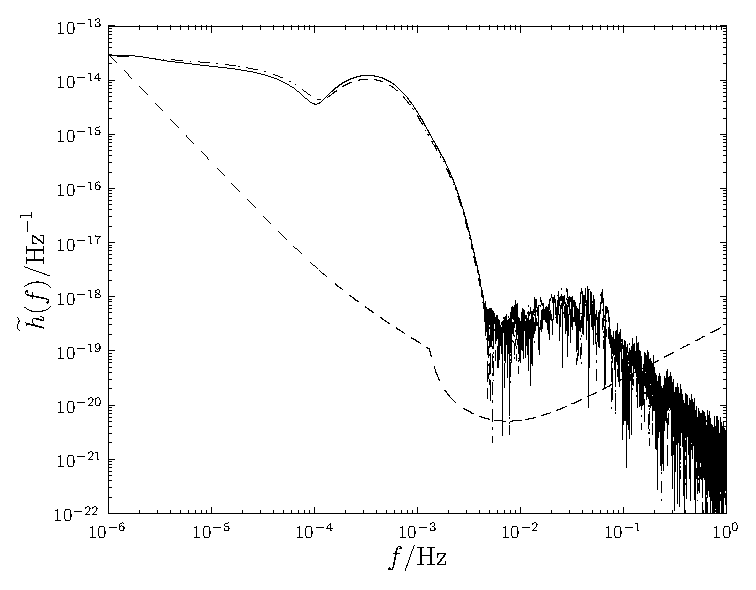
\includegraphics[width=0.45\textwidth]{Fig_new_sph_h_254}
\label{fig:Examples}
\caption{Waveform for $a_\ast \simeq 0.48$, $r_\mathrm{p} \simeq 8.8 r_\mathrm{g}$ and $\iota \simeq 2.0$. SNR is $\rho \simeq 2300$. The strain $\widetilde{h}_\mathrm{I}(f)$ is indicated by the solid line, $\widetilde{h}_\mathrm{II}(f)$ by the dot-dashed line, and the noise curve by the dashed line.}
  \end{center}
\end{figure}

The detectability of a burst depends upon its SNR $\rho$. The amplitude of the waveform is proportional to the CO mass $\mu$ and so $\rho$ is also proportional to $\mu$; we shall work in terms of a mass-normalised SNR
\begin{equation}
\hat{\rho} = \left(\frac{\mu}{M_\odot}\right)^{-1}\rho.
\end{equation}
We considered a range of orbits. The spin of the MBH and the orbital inclination were randomly chosen, and the periapse distance was set so that the distribution would be uniform in log-space (down to the point of the inner-most stable orbit). For each set of these extrinsic parameters, the periapse position, orientation of the MBH, and orbital position of the detector were varied: five random combinations of these intrinsic parameters (each being drawn from a separate uniform distribution) were used for each point. We take the mean of $\ln \rho$ for each set of randomised intrinsic parameters (starting position, MBH orientation and detector orientation).

There exists a correlation between the periapse radius and SNR, as shown in fig.~\ref{fig:SNR}.
\begin{figure}[ht!]
  \begin{center}
  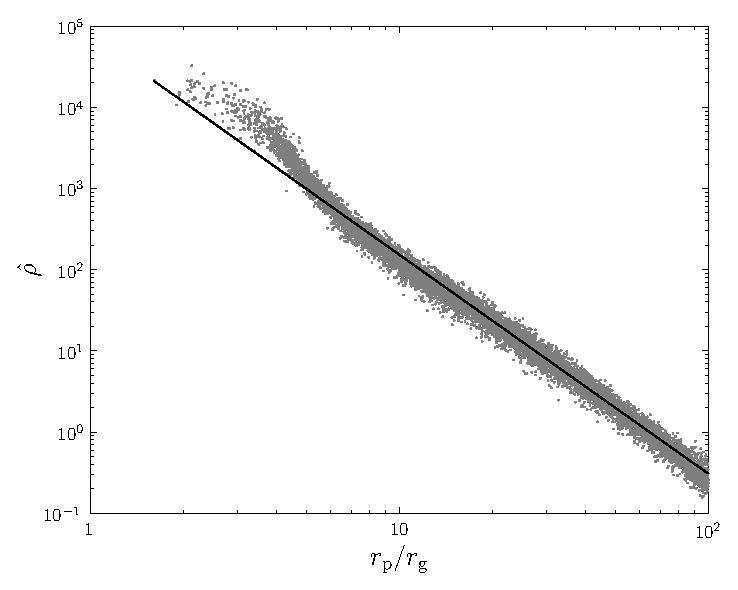
\includegraphics[width=0.45\textwidth]{Fig_SNR}
    \caption{Mass-normalised SNR as a function of periapse radius. The plotted points are the values obtained by averaging over each set of intrinsic parameters. The best fit line is $\log(\hat{\rho}) = -2.69\log(r_\mathrm{p}/r_\mathrm{g}) + 4.88$. This is fitted to orbits with $r_\mathrm{p} >  13.0 r_\mathrm{g}$ and has a reduced chi-squared value of $\chi^2/\nu = 1.73$.}
    \label{fig:SNR}
  \end{center}
\end{figure}
Closer orbits produce louder bursts. We have fitted a simple fiducial power law, as indicated by the straight line. The shape of the curve is predominately determined by the shape of the noise curve. The change in the trend reflects the change as we go from approximately power law behaviour into the bucket of the curve. Hence, we fit a power law to orbits with a characteristic frequency of $f_\ast = \sqrt{GM_\bullet/r_\mathrm{p}} < 1 \times 10^{-3}~\mathrm{Hz}$, so as to avoid spilling over into the bucket. Changing the cut-off within a plausible region alters the fit coefficients by around $0.1$.

Setting a detection threshold of $\rho = 10$, a $1 M_\odot$ ($10 M_\odot$) object would be expected to be detectable if the periapse distance is less than $27 r_\mathrm{g}$ ($65 r_\mathrm{g}$).

\section{Parameter estimation \& results}\label{sec:Estimation}

\subsection{Methodology}

Having detected a GW signal we are interested in what we can learn about the source. As an initial investigation we tried to use a Fisher matrix analysis. The Fisher matrix is a commonly used method of estimating the variance-covariance matrix and hence the precision to which parameters may be determined~\citep{Cutler1994}. The formalism is based upon the linearised-signal approximation~\citep{Vallisneri2008}. This should hold in the limit of high SNR. What constitutes high depends upon the waveform. Using the maximum-mismatch criterion of\citet{Vallisneri2008}, we found that bursts from the Galactic Centre could not be adequately described by the linearised-signal approximation, despite having what would be conventionally considered high SNR. This emphases the importance of checking the maximum-mismatch criterion.

As we cannot be confident in Fisher matrix results, we opted to instead to perform Markov chain Monte Carlo (MCMC) simulations. These are computationally more expensive, but more accurate. MCMC methods are widely used for inference problems; they are a family of algorithms used for integrating over a complicated probability distribution and are efficient for high-dimensional problems~\citep[chapter 29]{MacKay2003}. Parameter space is explored by constructing randomly a chain of $N$ samples. The distribution of points visited by the chain maps out the underlying distribution; this becomes asymptotically exact as $N \rightarrow \infty$.

To assess the convergence of the MCMC we check the trace plot (the parameters values throughout the run time of the chain) for proper mixing, that the one and two dimensional posterior plots fill out to a smooth distribution, and that the distribution widths tend towards consistent values.

\subsection{Data}

Waveforms were computed for a range of different orbits. In each case the massive black hole was assumed to have the standard MBH mass and position. The CO was chosen to be $10 M_\odot$, as the most promising candidates for EMRBs would be BHs: they are massive and hence produce higher SNR bursts, they are more likely to be on close orbits as a consequence of mass segregation~\citep{Bahcall1977, Alexander2009}, and they cannot be tidally disrupted. Orbits were chosen with periapses uniformly distributed in logarithmic space between the the innermost orbit and $16 r_\mathrm{g}$. The other parameters were chosen randomly from appropriate uniform distributions. 

The results of the MCMC runs illustrate why the Fisher matrix approach was insufficient. There are strong and complex parameter dependencies. For many sets of parameters the posteriors are far from Gaussian as assumed in the LSA.

It is possible to place good constraints from the closest orbits. These can provide sufficient information to give beautifully behaved posteriors although significant correlation between parameters persists.

Characteristic distribution widths are shown in fig.~\ref{fig:sigmas} for the mass and spin. Plotted is the standard deviation of the recovered posteriors. Filled circles are used for runs that appear to have converged. Open circles for those yet to converge, but which appear to be approaching an equilibrium state; widths should be accurate to within a factor of a few.

\begin{figure*}
\begin{center}
\subfigure[MBH mass $M_\bullet$ versus periapsis.]{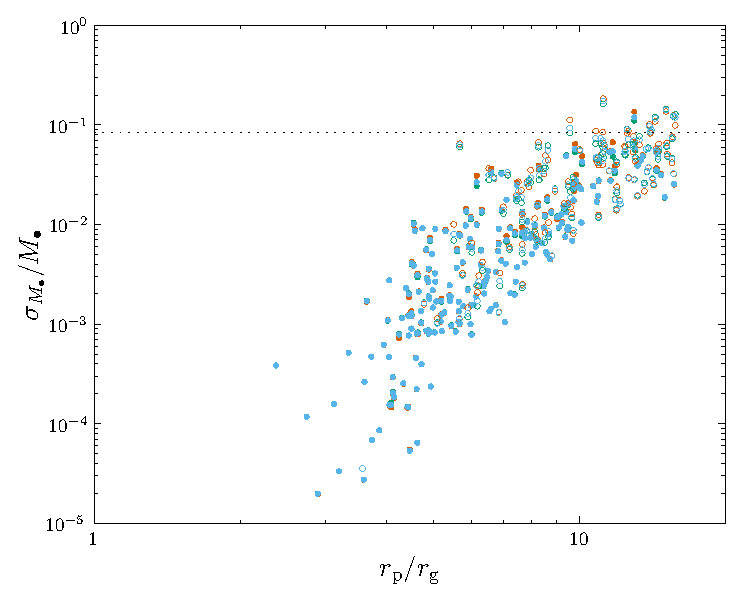
\includegraphics[width=0.44\textwidth]{Fig_MCMC_sigmas_rp_1}} \quad
\subfigure[MBH mass $M_\bullet$ versus SNR.]{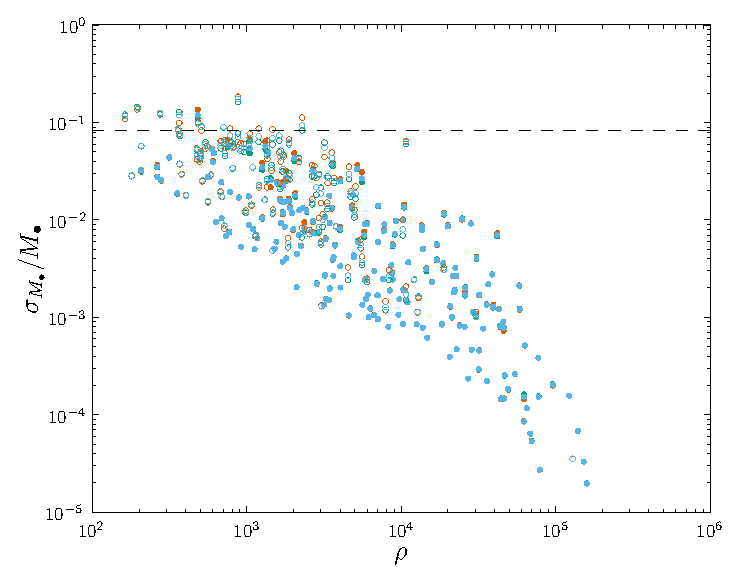
\includegraphics[width=0.45\textwidth]{Fig_MCMC_sigmas_SNR_1}} \\
\subfigure[MBH spin $a_\ast$ versus periapsis.]{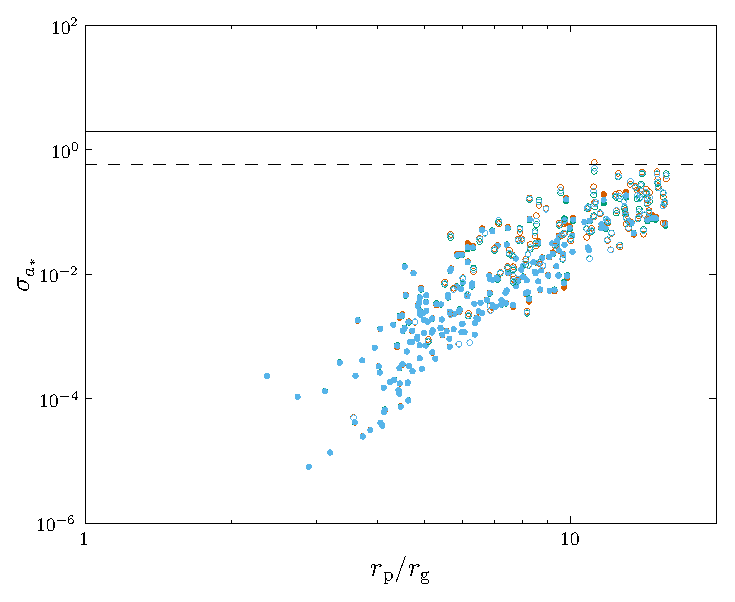
\includegraphics[width=0.44\textwidth]{Fig_MCMC_sigmas_rp_2}} \quad
\subfigure[MBH spin $a_\ast$ versus SNR.]{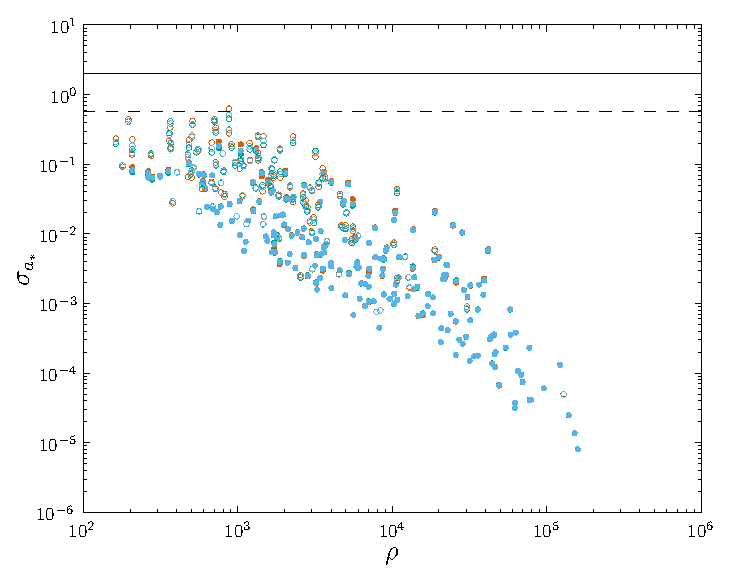
\includegraphics[width=0.45\textwidth]{Fig_MCMC_sigmas_SNR_2}} \\
\caption{Distribution widths as functions of periapse $r_\mathrm{p}$ and SNR $\rho$.. Filled circles are used for converged runs, open circles for those yet to converge. The dotted line indicates the current uncertainty for $M_\bullet$; the dashed lines the standard deviation for an uninformative prior, and the solid line the total prior range.}
\label{fig:sigmas}
\end{center}
\end{figure*}
These results do not incorporate any priors (save to keep them within realistic ranges). We have not folded in the existing information we have, for example, about the MBH's mass. Therefore, the resulting distributions characterise what we could learn from EMRB's alone. By the time a space-borne GW detector finally flies, we may well have much better constraints on some of the parameters.

The widths show a general trend of decreasing with decreasing periapsis or increasing SNR, but there is a large degree of scatter. There does not appear to be a strong dependence upon any single input parameter, with the exception of the spin. The widths for $\iota$, $\Theta_\mathrm{K}$, $\Phi_\mathrm{K}$, $\phi_\mathrm{p}$ and $\chi_\mathrm{p}$ all increase for smaller spin magnitudes. These parameters are all defined with reference to the coordinate system established by the direction of the spin axis: for $a_\ast = 0$ we have spherical symmetry and there would be ambiguity in defining them.

\subsection{Scientific potential}

The current uncertainty in the mass is $\sigma_{M_\bullet} = 0.36 \times 10^6 M_\odot$ ($\sim 8\%$). There are few runs amongst our data set that are not better than this: it appears that orbits of a $\mu = 10 M_\odot$ CO with periapses $r_\mathrm{p} \lesssim 13 r_\mathrm{g}$ should be able to match our current observational constraints. Accuracy of $1\%$ could be possible if $r_\mathrm{p} \lesssim 8 r_\mathrm{g}$.

The spin is less well constrained. To obtain an uncertainty for the magnitude of $0.1$, comparable to that achieved in X-ray measurements of active galactic nuclei, it appears that the periapsis needs to be $r_\mathrm{p} \lesssim 11 r_\mathrm{g}$. For smaller periapses, the uncertainty can be much smaller, indicating that an EMRB could be an excellent probe. The orientation angles for the spin axis may be constrained to better than $0.1$ for $r_\mathrm{p} \lesssim 11 r_\mathrm{g}$. It may well be possible to learn both the direction and the magnitude of the spin. This could illuminate the MBH's formation, as the spin encodes information of the merger and accretion history.

We have no {\it a priori} knowledge about the CO or its orbit, so anything we learn would be new. However, this is not particularly useful information, unless we observe multiple bursts, and can start to build up statistics for the dynamics of the GC. Using current observations for the distance to the GC, which could be further improved by the mass measurement from the EMRB, it is possible to infer a value for the mass $\mu$ from $\zeta$. This could inform us of the nature of the object (BH, NS or WD) and be a useful consistency check. A small value of $\zeta$, indicating a massive CO would be unambiguous evidence for the existence of a stellar mass black hole.

\bibliography{Parabolic}
\bibliographystyle{asp2010}

\end{document}

% toto
% tata
